\documentclass[../main.tex]{subfiles} 
\begin{document}
	A arquitetura implementada efetivamente em VHDL pode ser observada pelo RTL da figura~\ref{fig:bloco_dados_RTL}.
	
	\begin{figure}[H]
		\centering
		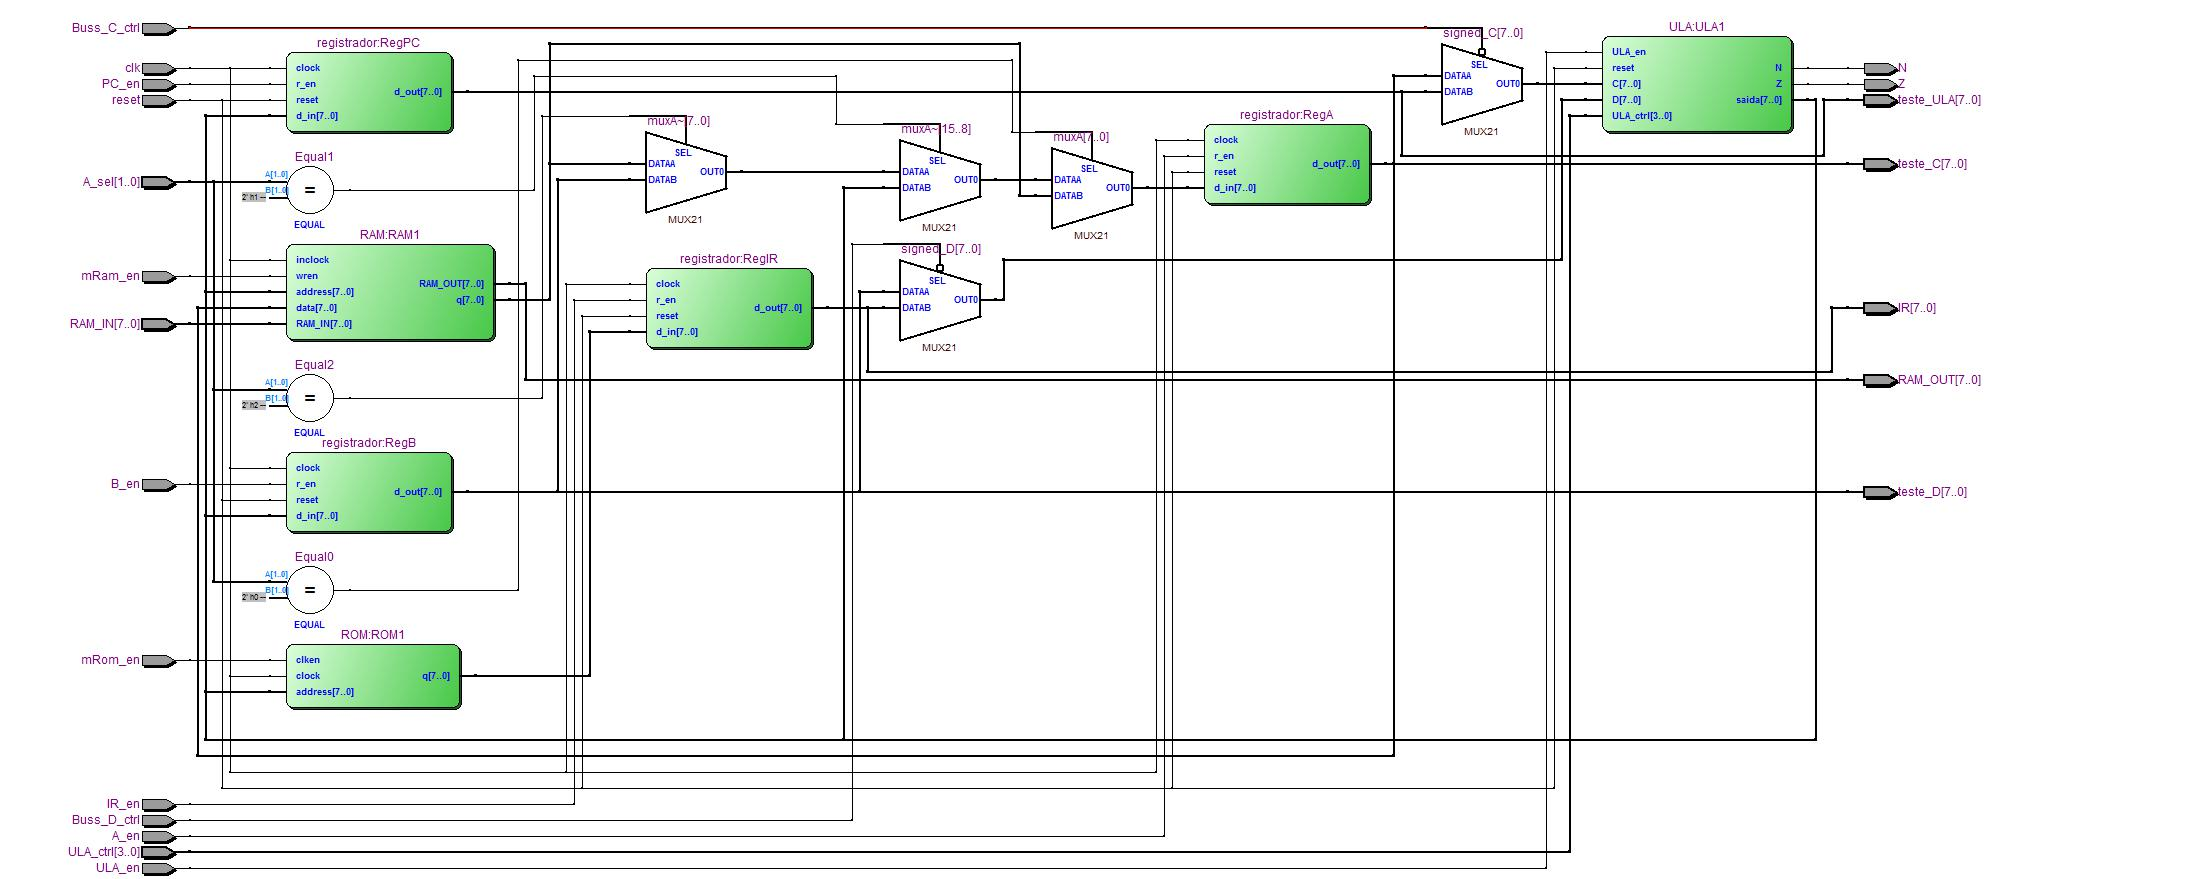
\includegraphics[width=\textwidth]{img/bloco_dados_RTL}
		\caption{Arquitetura implementada em VHDL para o Bloco de Dados.}
		\label{fig:bloco_dados_RTL}
	\end{figure}
	
	Os principais pontos que diferem do projeto inicial (figura~\ref{fig:arq_bloco_dados}) do implementado são:
	\begin{itemize}
		\item \A{} só grava o dado na borda de descida do clock (\textit{not\_clk}). Esta implementação foi feita para facilitar o tratamento de funções como \textit{SWP} evitando a necessidade de passos adicionais;
		\item \A{} recebe sinais advindos, além da ULA e da RAM, do registrador \B{}. Esta alteração no multiplexador de entrada de \A{} foi realizada para implementar mais facilmente a função \textit{SWP};
		\item Os barramentos de dados C e D passam a ser controlados por multiplexadores em vez dos \textit{tristates} de saída dos registradores. Esta medida foi tomada para reduzir a quantidade de sinais de controle.
		\item Foi colocado um sinal de enable de saída na ULA (\textit{ULA\_en}) posibilitando o comportamento de latch da mesma;
		\item Foram acrescentados sinais de reset em todos os componentes a fim de garantir uma correta inicialização do processador;
		\item Foram implementados sinais extras a fim de facilitar o \textit{debug} e a análise da simulação;
	\end{itemize}
	
	Para cada uma das subsseções abaixo foi criado um novo projeto de hardware em VHDL e foi montado um \textit{testbench}
	baseado em estímulos gerados por arquivos \textit{.vhd}.
	
	A estrutura final do Bloco de Dados foi montada usando a estrutura de \textit{COMPONENTS} e \textit{PORT MAP}, excetuando-se
	alguns multiplexadores que foram implementados utilizando lógica \textit{IF-THEN-ELSE}.
	
	\subsection{ULA}
		\label{sec:ULA}
		As operações implementadas pela ULA são descritas na tabela~\ref{tab:comandos_ULA}.
		\begin{table}[H]
			\centering
			\caption{Funções implementadas na ULA}
			\begin{tabular}{|l|c|c|l|} %4 colunas
			\hline
			Função & Código & Instruções que utilizam & Descrição					 		\\\hline
			PASSA\_C 	& 0b0000 	& Todas		&	Passa o conteúdo de C para saída da ULA	\\\hline
			PASSA\_D 	& 0b0001 	& Todas		&	Passa o conteúdo de D para saída da ULA	\\\hline
			INC\_C 		& 0b0110 	& Todas		&	Incrementa 1 no conteúdo de C			\\\hline
			C AND D 	& 0b0010 	& AND		&	Executa operação AND entre C e D		\\\hline
			C OR D 		& 0b0011 	& OR		&	Executa operação OR entre C e D			\\\hline
			NOT C 		& 0b0100 	& NOT		&	Executa operação inversão de bits com C	\\\hline
			$C+D$ 		& 0b0101 	& ADD		&	Soma C com D (Complemento de 2)			\\\hline						
			$C-D$ 		& 0b1001 	& BEQ, BLT	&	Subtrai D de C (Complemento de 2)		\\\hline
			$C*D$ 		& 0b1010 	& MUL		&	Armazena $C*D$ num registrador interno	\\\hline						
			$LSB(C*D)$	& 0b0111 	& MUL		&	Passa os 8 primeiros bits de $C*D$		\\\hline						
			$HSB(C*D)$	& 0b1000 	& MUL		&	Passa os 8 últimos bits de $C*D$		\\\hline						
			DEC\_C		& 0b1011 	& HALT		&	Decrementa 1 no conteúdo de C			\\\hline						
			\end{tabular}
			\label{tab:comandos_ULA}
		\end{table}
		
		Os flags Z(indicando zero) e N(indicando números negativos) na ULA são tratados em processos assíncronos 
		e estão ativos sempre que a saída da ULA estiver ativa.
		
		As operações aritiméticas são realizadas baseadas na biblioteca \textit{IEEE.numeric\_std} com sinais do tipo
		\textit{SIGNED}.
	\subsection{RAM}
		\label{sec:RAM}
		A memória RAM foi desenvolvida com o auxílio da ferramenta \textit{Mega Wizard} do \textit{Quartus 12.3}, sendo composta por: 
		256 palavras de 8 bits (equivale a 8 bits de endereçamento); uma saída de dados; uma entrada de endereçamento; uma entrada de dados; e uma entrada de enable de gravação.
		
		O mapeamento da memória foi feito utilizando lógica \textit{IF-THEN-ELSE}, diretamente no arquivo gerado pelo \textit{Mega Wizard}.
	\subsection{ROM}
		\label{sec:ROM}
		A memória ROM foi desenvolvida com o auxílio da ferramenta \textit{Mega Wizard} do \textit{Quartus 12.3}, sendo composta por:
		256 palavras de 8 bits (equivale a 8 bits de endereçamento); uma saída de dados; uma entrada de endereçamento; e uma entrada de habilitação de saída de dados.
		
		Sempre um Ciclo de Clock antes de \IR{} ler da ROM, é necessário habilitar a saída de dados da mesma.
		
		O programa é gravado na ROM através de um arquivo de inicialização com extensão \textit{.mif} como exemplificado posteriormente na seção~\ref{sec:simulacao}.
		
	\subsection{Registradores}
		\label{sec:registradores}
		
		Todos os registradores desenvolvidos são estruturas simples seguindo a mesma filosofia dos registradores desenvolvidos pelo
		treinamento \textit{Altera} reproduzido em aula.
\end{document}